\documentclass{article}

\usepackage{graphicx}
\usepackage{tikz}
\usepackage{tikzsymbols}
\usetikzlibrary{calc,patterns,shapes.geometric}
\pagestyle{empty}
\usepackage[margin=0pt]{geometry}
\geometry{papersize={14in,12in}}

\def\centerarc[#1](#2)(#3:#4:#5){\draw[#1] ($(#2)+({#5*cos(#3)},{#5*sin(#3)})$) arc (#3:#4:#5);}

\begin{document}
	\begin{figure}
		\centering
		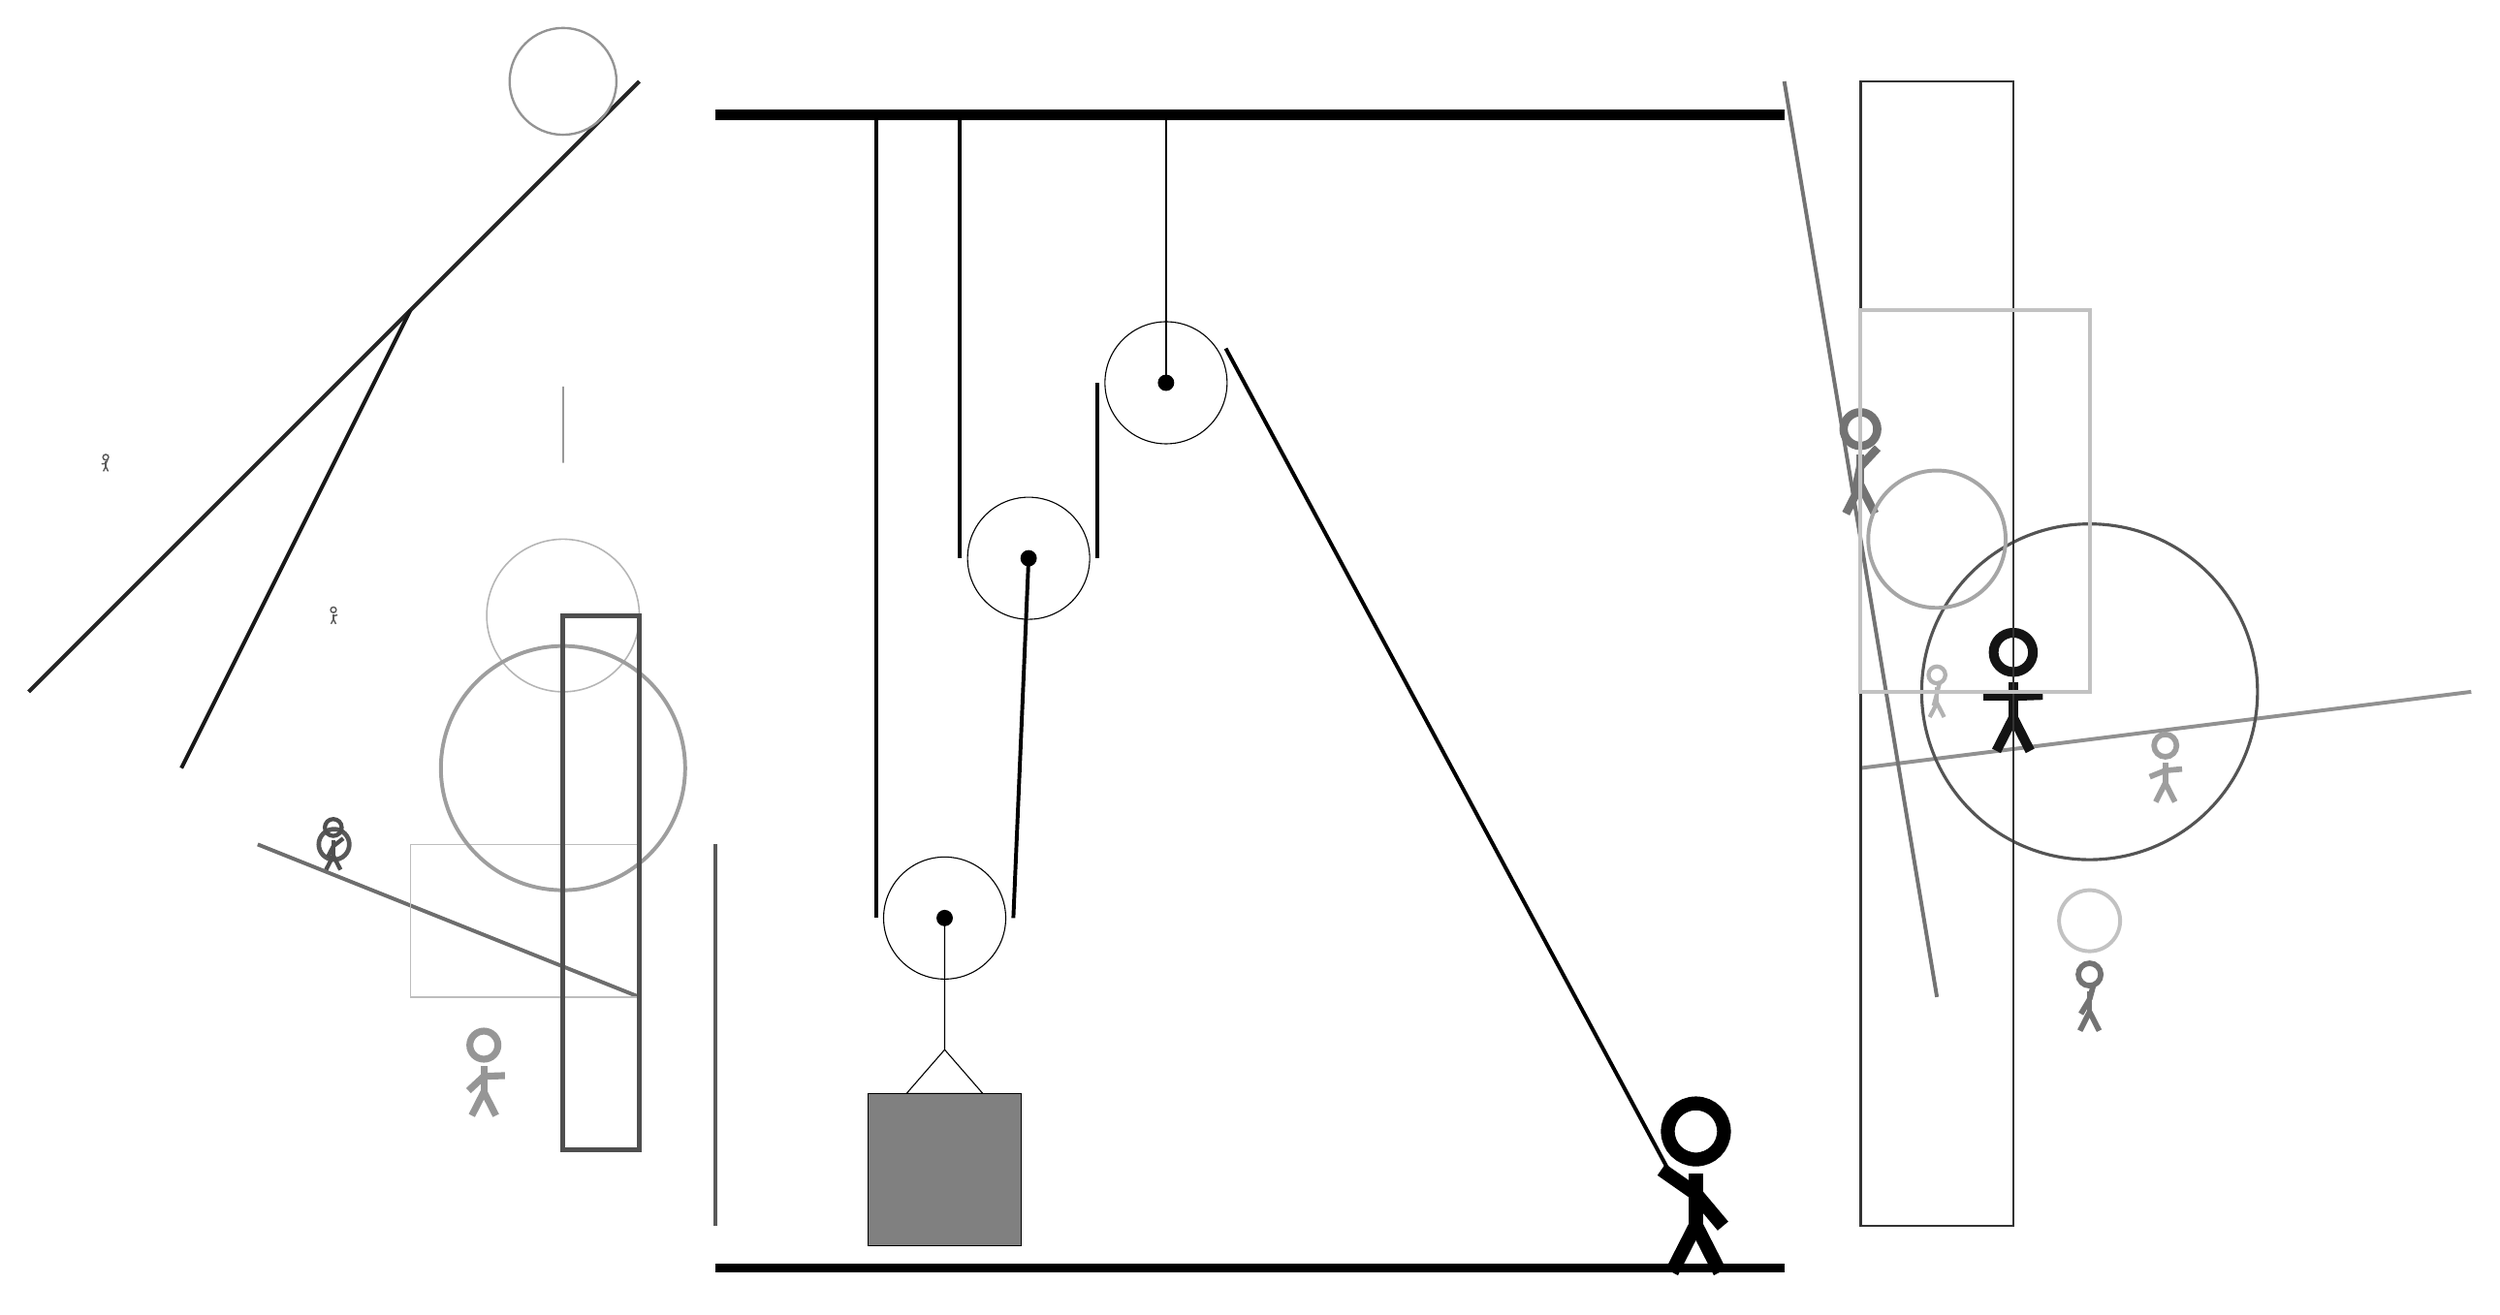
\begin{tikzpicture}
			%%%%% START %%%%%
			
			\draw[fill=black] (-2, 11.5) rectangle (12, 11.625);
			
			\draw (1, 1.035) circle (0.8);
			\draw[fill=black] (1, 1.035) circle (0.1);
			
			\draw (2.1, 5.75) circle (0.8);
			\draw[fill=black] (2.1, 5.75) circle (0.1);
			
			\draw (3.9, 8.05) circle (0.8);
			\draw[fill=black] (3.9, 8.05) circle (0.1);
			\draw[thick] (3.9, 8.05) -- (3.9, 11.5);
			
			\draw [line width=0.6mm, color=black!65](-7, 2) circle (0.2);
			
			\node[line width=0.4mm, color=black!30] at (14, 4) {\Strichmaxerl[3][75][76]};
			\draw[line width=0.5mm, color=black!43](13, 3) -- (21, 4);
			\node[line width=0.2mm, color=black!65] at (-10, 7) {\Strichmaxerl[1][6][64]};
			
			\draw[line width=0.5mm, color=black!57](-3, 0) -- (-8, 2);
			\draw[line width=0.2mm, color=black!26] (-3, 0) rectangle (-6, 2);
			\draw[line width=0.5mm, color=black!85](-3, 12) -- (-11, 4);
			
			\draw [line width=0.2mm, color=black!29](-4, 5) circle (1.0);
			\draw [line width=0.5mm, color=black!38](-4, 3) circle (1.6);
			\node[line width=0.6mm, color=black!38] at (17, 3) {\Strichmaxerl[4][22][5]};
			\draw [line width=0.3mm, color=black!42](-4, 12) circle (0.7);
			\draw[line width=0.5mm, color=black!90](-6, 9) -- (-9, 3);
			\node[line width=0.2mm, color=black!55] at (13, 7) {\Strichmaxerl[6][78][47]};
			
			\node[line width=0.6mm, color=black!69] at (-7, 2) {\Strichmaxerl[3][63][38]};
			\draw [line width=0.4mm, color=black!67](16, 4) circle (2.2);
			\node[line width=0.7mm, color=black!55] at (16, 0) {\Strichmaxerl[4][59][75]};
			
			\node[line width=0.4mm, color=black!41] at (-5, -1) {\Strichmaxerl[5][43][2]};
			
			\draw [line width=0.5mm, color=black!35](14, 6) circle (0.9);
			\draw[line width=0.5mm, color=black!65](-2, 2) -- (-2, -3);
			\node[line width=0.4mm, color=black!92] at (15, 4) {\Strichmaxerl[7][0][2]};
			\draw[line width=0.2mm, color=black!40] (-4, 8) rectangle (-4, 7);
			\draw[line width=0.5mm, color=black!55](12, 12) -- (14, 0);
			
			\draw [line width=0.5mm, color=black!24](16, 1) circle (0.4);
			\draw[line width=0.3mm, color=black!80] (13, -3) rectangle (15, 12);
			\draw[line width=0.5mm, color=black!24] (13, 9) rectangle (16, 4);
			
			\draw[line width=0.6mm, color=black!69] (-3, -2) rectangle (-4, 5);
			\node[line width=0.2mm, color=black!65] at (-7, 5) {\Strichmaxerl[1][90][17]};
			
			\draw (1, 1.035) -- (1, -0.69) -- (0.5, -1.265) -- (1.5, -1.265) -- (1, -0.69);
			\draw[fill=black!50] (0, -1.265) rectangle (2, -3.265);
			
			\draw[line width=0.5mm] (0.1, 11.5) -- (0.1, 1.035);
			\centerarc[line width=0.5mm](1, 1.035)(180:360:0.9);
			\draw[line width=0.5mm](1.9, 1.035) -- (2.1, 5.75);
			\draw[line width=0.5mm] (1.2, 11.5) -- (1.2, 5.75);
			\centerarc[line width=0.5mm](2.1, 5.75)(180:360:0.9);
			\draw[line width=0.5mm](3.0, 5.75) -- (3.0, 8.05);
			\centerarc[line width=0.5mm](3.9, 8.05)(30:180:0.9);
			\draw[line width=0.5mm] (4.683, 8.5) -- (10.5, -2.3);
			
			\node at (10.8, -2.5) {\Strichmaxerl[10][-35][-50]};
			
			\draw[fill=black] (-2, -3.5) rectangle (12, -3.6);
			
			%%%%% END %%%%%
		\end{tikzpicture}
	\end{figure}	
\end{document}